%
% File: chap01.tex
% Author: Victor F. Brena-Medina
% Description: Introduction chapter where the biology goes.
%
\let\textcircled=\pgftextcircled

\chapter{Conceptual Framework}
\label{chap:conceptualFramework}
\initial{M}obile applications have changed the way we interact with the world around us, now we don't rely on a desktop and constant refreshing of web applications to get the data we need to start our day, nor do we need to stay put in a place with wired connections since we can get our data on the go. Mobile apps help get your data customized by the vendor without having to worry about the device or hardware underneath it, this abstraction helps developers code applications that will work in a wide variety of mobile phones.

As it was in the 1990's with the rise of desktop computers into mainstream use, the market was bombarded with multiple viruses, worms and trojans aimed at users in order to steal, forge, or otherwise break the system it infected. This trend has now caught up to mobile phones, the new frontier.

As of now there are really only two key players in the mobile world, Google and Apple, and both have similar ecosystems with gaping difference in how they approach security.
While Apple's approach is to have an App Store where all apps that are published can be downloaded with a press of a button. But before being allowed inside the App Store, an aspiring app must have passed a rigorous testing and verification by Apple, in which they must abide by their terms and license agreement.

Google's approach varies significantly, any developer who wishes to publish into the play store, can do so without a mainstreamed verification process. Google checks apps for security before they enter the Android Market, but there isn’t an Android security policy to which all those apps adhere. Android uses sandboxing, which limits how an app can interact with other apps and the OS, thus limiting the effects of any malware as well. But some Android phone malware is designed to trick users into lifting these limits, by presenting seemingly authentic requests for permission to access other apps and OS components. A virus can then use these permissions to attack the full mobile platform. For the most part, Android app security is good, but the chance for malicious apps to make their way into the Android Market is still present \cite{techtarget}.



% \initial{A} tool for reverse engineering 3rd party, closed, binary Android apps. It can decode resources to nearly original form and rebuild them after making some modifications. It also makes working with an app easier because of the project like file structure and automation of some repetitive tasks like building apk, etc.

% It is NOT intended for piracy and other non-legal uses. It could be used for localizing, adding some features or support for custom platforms, analyzing applications and much more.

%=======
\section{Android OS}
\label{sec:01androidos}
Android is an open source, Linux-based software stack created for a wide array of devices and form factors. The following diagram shows the major components of the Android platform.

\begin{figure}[h]
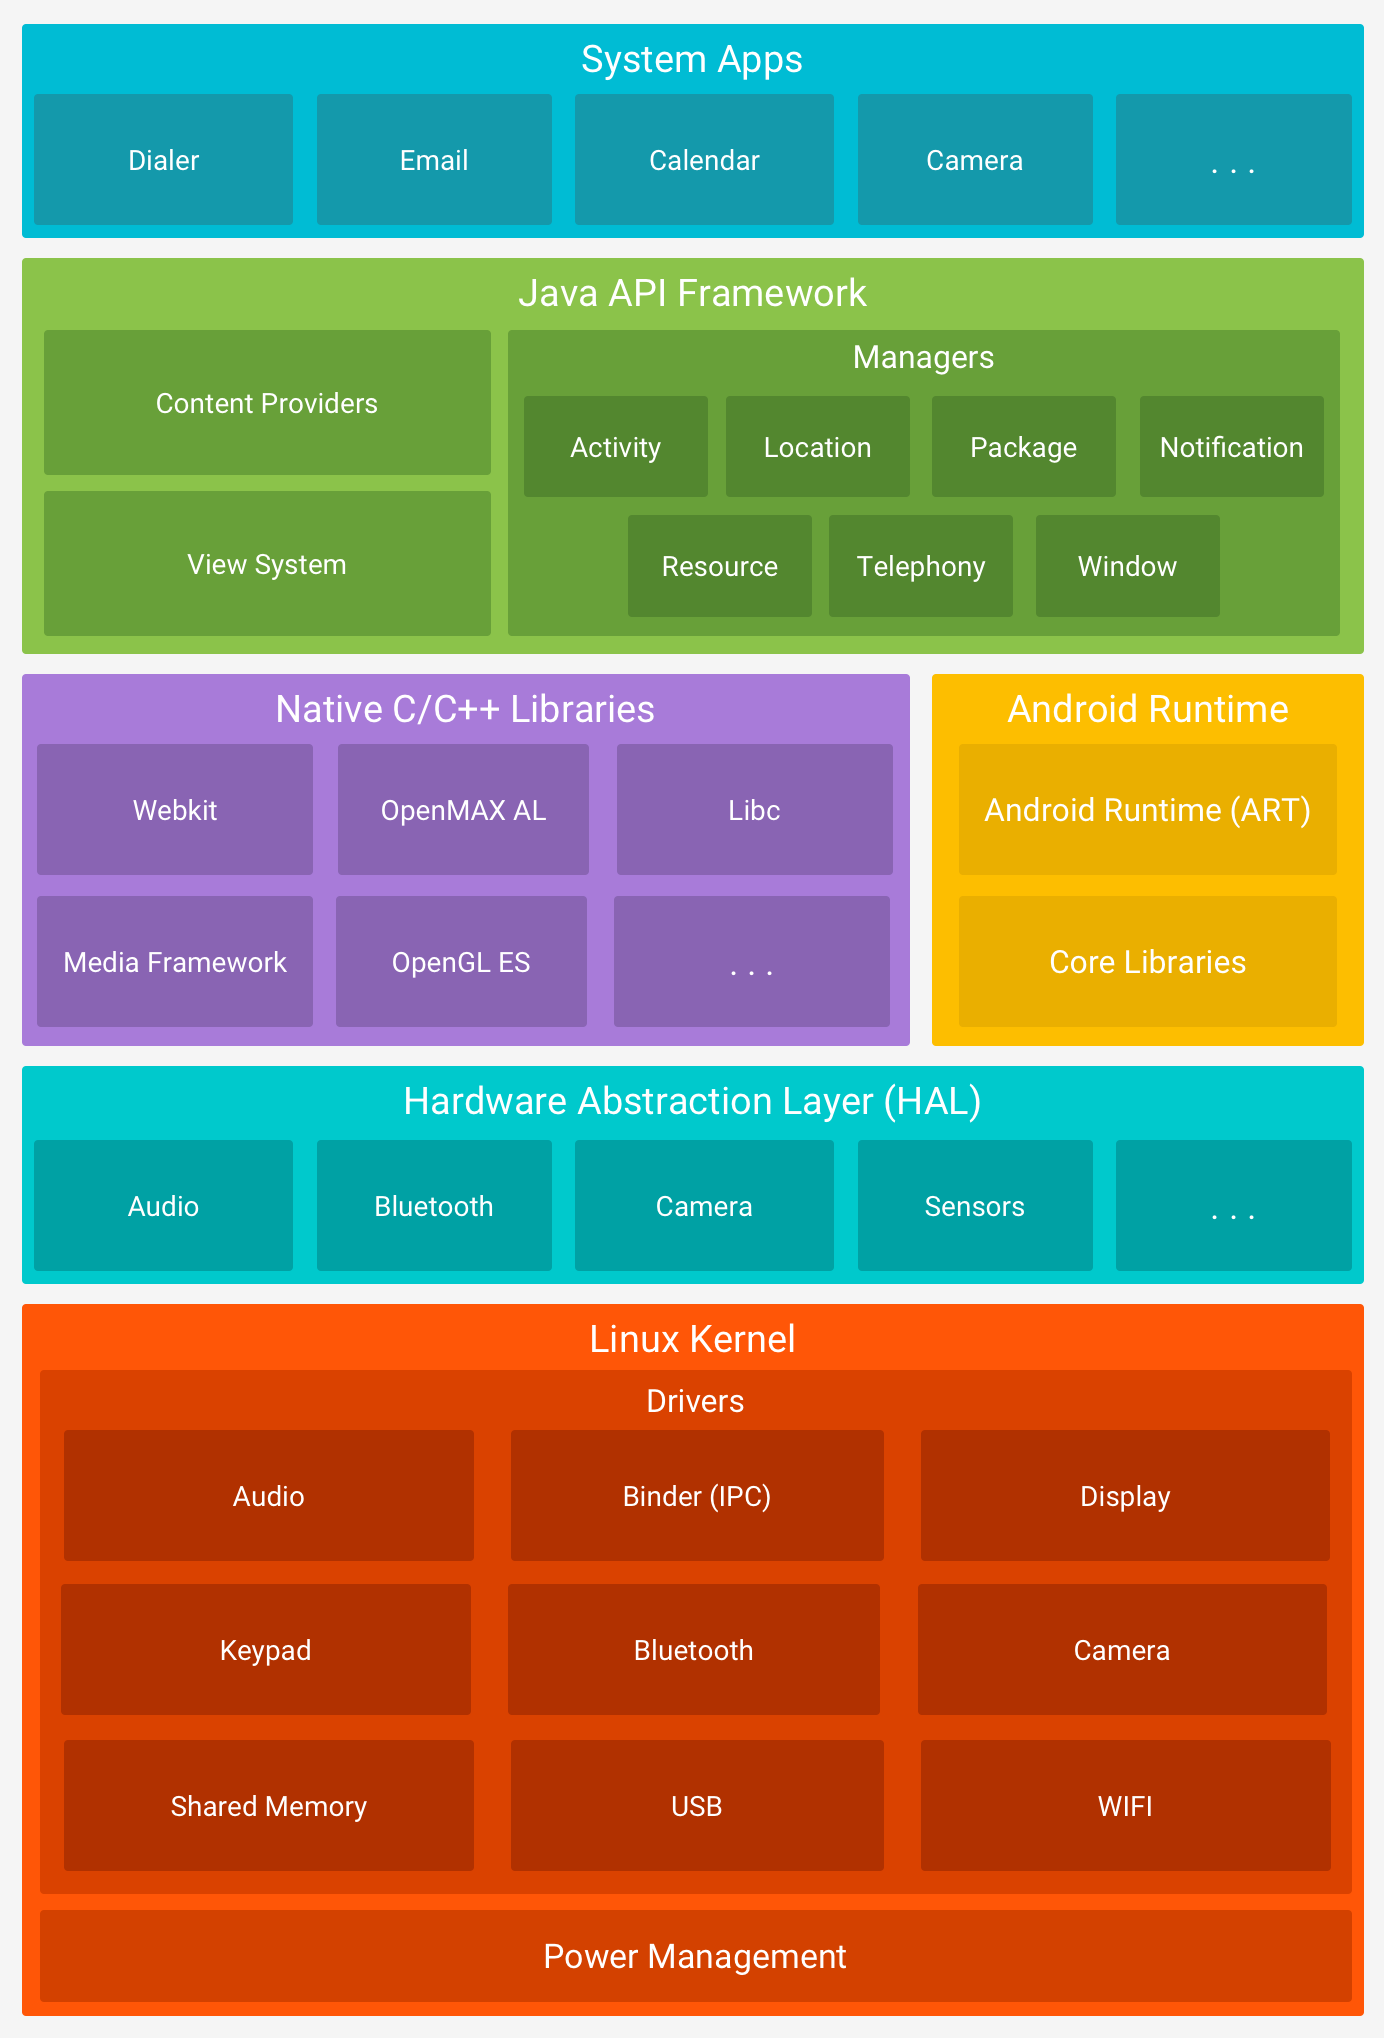
\includegraphics[scale=0.18]{img/android-stack_2x.png}
\centering
\caption{Android Stack}
\end{figure}

\subsection{Linux Kernel}

The foundation of the Android platform is the Linux kernel. For example, the Android Runtime (ART) relies on the Linux kernel for underlying functionalities such as threading and low-level memory management.

Using a Linux kernel allows Android to take advantage of key security features and allows device manufacturers to develop hardware drivers for a well-known kernel.

\subsection{Hardware Abstraction Layer (HAL)}
The hardware abstraction layer (HAL) provides standard interfaces that expose device hardware capabilities to the higher-level Java API framework. The HAL consists of multiple library modules, each of which implements an interface for a specific type of hardware component, such as the camera or bluetooth module. When a framework API makes a call to access device hardware, the Android system loads the library module for that hardware component.

\subsection{Android Runtime}
For devices running Android version 5.0 (API level 21) or higher, each app runs in its own process and with its own instance of the Android Runtime (ART). ART is written to run multiple virtual machines on low-memory devices by executing DEX files, a bytecode format designed specially for Android that's optimized for minimal memory footprint. Build tool chains, such as Jack, compile Java sources into DEX bytecode, which can run on the Android platform.

Prior to Android version 5.0 (API level 21), Dalvik was the Android runtime. If your app runs well on ART, then it should work on Dalvik as well, but the reverse may not be true.

\subsection{Native C/C++ Libraries}

Many core Android system components and services, such as ART and HAL, are built from native code that require native libraries written in C and C++. The Android platform provides Java framework APIs to expose the functionality of some of these native libraries to apps. For example, you can access OpenGL ES through the Android framework’s Java OpenGL API to add support for drawing and manipulating 2D and 3D graphics.

\subsection{Java API Framework}
The entire feature-set of the Android OS is available through APIs written in the Java language. These APIs form the building blocks needed to create Android apps by simplifying the reuse of core, modular system components and services.

\section{Mobile Applications}
\label{sec:01mobileapp}
The Android platform suffers the issue of fragmentation -- there are multiple versions of Android in the market, even on current devices. Manufacturers often make their own changes to Android, so they could be behind Google's current reference release. In addition, carriers and manufacturers may not update their devices' Android version when Google does, or they take months or even years to do so.

As a result, many people within the same organization might be using outdated versions that could be riddled with security vulnerabilities. People focus on malware risks of Android, but arguably the greater risk is that fragmentation creates different user experiences, this variety of user experiences makes it hard to educate employees about how to take security measures, because the experience on each device is different. As a result many multiple users end up with different versions of Android which in turn means different versions of any one application.

This difference between versions means that users could be vendor locked into a version of android, for example Samsung has statistically released the next flavor of Android about 6-10 months after Google has released it, leaving users open to attack during this wide window of not being able to get the latest updates and patches.

Any developer suffers the consequences of this delay, from a security standpoint , they must now version an application to be able to support multiple versions of the Android OS, keeping new features off a specific version , etc. 

\section{Threats and Risks in the Android Eco System}
Google has placed numerous measures in order to keep apps as secure as possible, one the main security pillars is the Android Security Sandbox (AAD) , which isolates app data and code execution from other apps, it is an application framework with robust implementations of common security functionality such as cryptography, permissions, and secure Inter Process Communication (IPC).

Even though Android makes it easy to publish apps to the Play Store, it makes it way to easy to publish malicious applications, in order to attempt to prevent this a security measure from 2010 that is still in effect today is that every application has to be signed before being installed on a device, but in order to circumvent this, a hacker may use a self signed certificate before publishing to the Play Store, even more appalling is the fact that users may also download apps from third party stores such as slideme.org and androidlib.com.

Apps can't just be installed and access every component of the phone, mainly because of the sandboxing mentioned earlier. In order to achieve full compromise, the user must allow and application permissions, these permissions are defined in advanced by the developer (in a file called AndroidManifest.xml) and the user is prompted with the permission requirements of the app before installation.



\section{How to prevent mobile threats}
There is no silver bullet that can prevent security breaches in the software world, and Android is no different. Preventing reverse engineering on an application is not 100\% possible but it be slowed down quite a bit, techniques such as obfuscation make understanding and modifying the underlying code much harder (but not impossible). In the end, one has to understand that an application can't be protected from modifications and any protections in place can be disabled or removed.

That being said, there are numerous methods for preventing mobile threats such as
\begin{enumerate}
	\item{Usage of tools like ProGuard. These will obfuscate the code, and make it harder to read when decompiled, if not impossible}
	\item{Move the most critical parts of the service out of the app, and into a webservice, hidden behind a server side language like PHP or use the NDK to write them natively into .so files, which are much less likely to be decompiled than apks. Decompiler for .so files don't even exists as of now (and even if they did, it wouldn't be as good as the Java decompilers). Finally the usage of SSL/TLS when interacting between the server and device is mandatory for securing communication.}
	\item{When storing values on the device, don't store them in a raw format, but instead use an algorithm to calculate the real value. Although this approach does in a way protect against tampering to obtain actual values (an attacker can still modify the entry value and get random results) it is not a security measure.}
	\item{In cases of payment processing apps, sending of raw data is not always the most secure way of processing the data, one approach to prevent interception or modification of values being sent to the server is to have base values that add up to the final value, for example, instead of sending the value 1000 to the server, the value is decomposed into smaller numbers that are assigned to strings, so 1000 could be decomposed as 10*10+100*4+500*1 and the numbers 10,100, and 500 are not sent as number but as names of people such as 10 = Daniel , 100 = Max, 500 = Bob and so on and the backend knows the conversion from string to number. This prevents a hacker from sending values to the endpoint and makes it harder to understand what is happening}
	\item{Insertion of random bits of code that has no meaning in an attempt to confuse whomever is trying to reverse engineer the application. Common practice is to insert classes that will catch the attention of anyone who is looking at the code, for example , compiling classes that generate a Fibonacci sequence called CreditCard.java is guaranteed to make the attacker waste valuable time. }
\end{enumerate}

\subsection{Requirements}

The application requires only Java 1.7 (JRE 1.7) and some basic knowledge of Android SDK, AAPT and the Smali language alongside some in depth understanding of computer architecture, assembler and hexadecimal numbers.

\subsection{Installation}

 The first library to install is the ia32-libs if the system is running on top a x64 architecture and install the apktool script and the apktool.jar and move both of them to a directory that is in the \$PATH variable, for example the /usr/lib/bin directory.



% \label{subsec:subsec01}

% Begins a subsection.

% %A figures matrix.
% \begin{figure}[t!]
% \centering
% \begin{minipage}{3.3cm}
%     \centering
%     \subtop[]{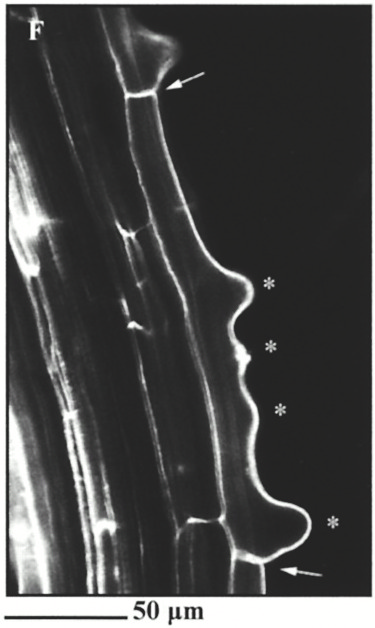
\includegraphics[height=0.28\textheight]{fig01/Nswellings}\label{sf:multiRH02a}}
% \end{minipage}
% \hspace{0.5cm}
% \begin{minipage}{3.3cm}
%     \centering
%     \subtop[]{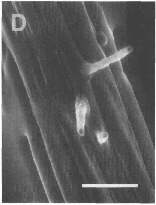
\includegraphics[height=0.27\textheight]{fig01/Mswellings}\label{sf:multiRH02b}}
% \end{minipage}
% \hspace{1.3cm}
% \begin{minipage}{3.3cm}
%     \centering
%     \subtop[]{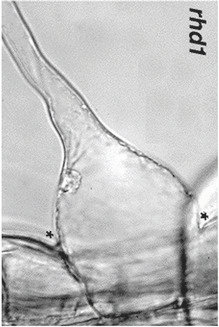
\includegraphics[height=0.27\textheight]{fig01/rhd1}\label{sf:multiRH02c}}
% \end{minipage}
% \\ \vspace{0.1cm}
% \begin{minipage}{10cm}
%     \centering
%     \subtop[]{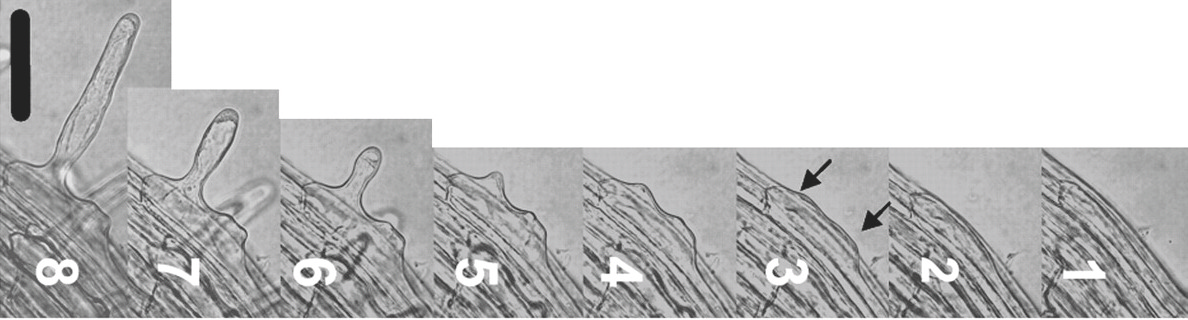
\includegraphics[height=0.145\textheight]{fig01/mutantrhd6}\label{sf:multiRH02d}}
% \end{minipage}
% \\ \vspace{0.1cm}
% \begin{minipage}{10cm}
%     \centering
%     \subtop[]{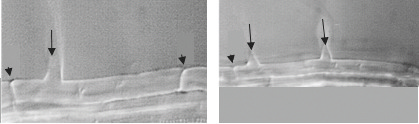
\includegraphics[height=0.16\textheight]{fig01/auxab}\label{sf:multiRH02e}}
% \end{minipage}
% \mycaption[Hair-forming mutant cells.]{(a) A mutant RH cell. Asterisks show multiple sites of RH initiation in a single root hair cell (indicated by the arrows). Figure reproduced from \cite{rigas01}. (b)~Hair-forming cell with three RH initiation locations. The bar represents $50\mu m$. Figure reproduced from \cite{massuci01}. (c) Large bump in mutant {\itshape rhd1}. Figure reproduced from \cite{griersonRH}. (d) Mutant overexpressing gene {\itshape ROP2}; from right-hand to left-hand, numbers indicate progressive snapshots at different times. RH initiation sites are indicated by the arrows. The bar represents $75\mu m$. Figure reproduced from~\cite{mjones01}. (e)~Mutants affected by auxin. On the left-hand side, RH site is farther away from the apical end (left arrow cap); on the right-hand side, multiple RH locations (arrows). Figure reproduced from~\cite{payne01}.}
% \label{fig:multiRH02}
% \end{figure}

% % A single figure
% \begin{figure}[t!]
%   \centering
%   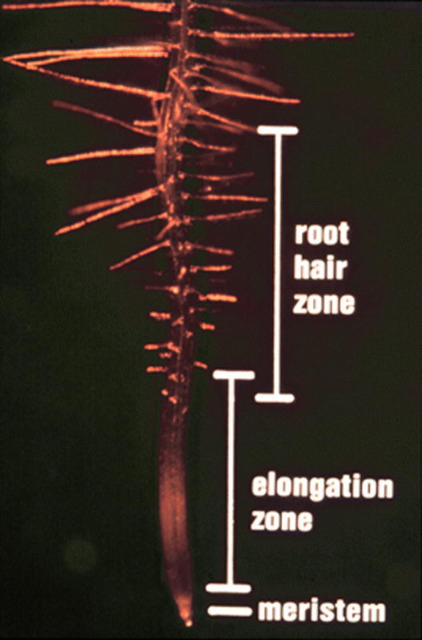
\includegraphics[height=0.35\textheight]{fig01/devepzones}
%   \mycaption[Developmental zones of an Arabidopsis root.]{Developmental zones of an Arabidopsis root. Figure reproduced from \cite{griersonRH}.}
%   \label{fig:RHP02}
% \end{figure}

%=========================================================